\begin{mybilan}
	\begin{itemize}
		\item Pendant un changement d'état d'un corps, sa \kw{masse ne varie pas}, mais son \kw{volume change}.
		\item La \kw{solidification} est le passage de \kw{l'état liquide à l'état solide}.
		\item La \kw{vaporisation} est le passage de \kw{l'état liquide à l'état gazeux}.
		\item La \kw{fusion} est le passage de \kw{l'état solide à l'état liquide}.
		\item La \kw{liquéfaction} est le passage de \kw{l'état gazeux à l'état liquide}.
		
	\end{itemize}

	\begin{center}
		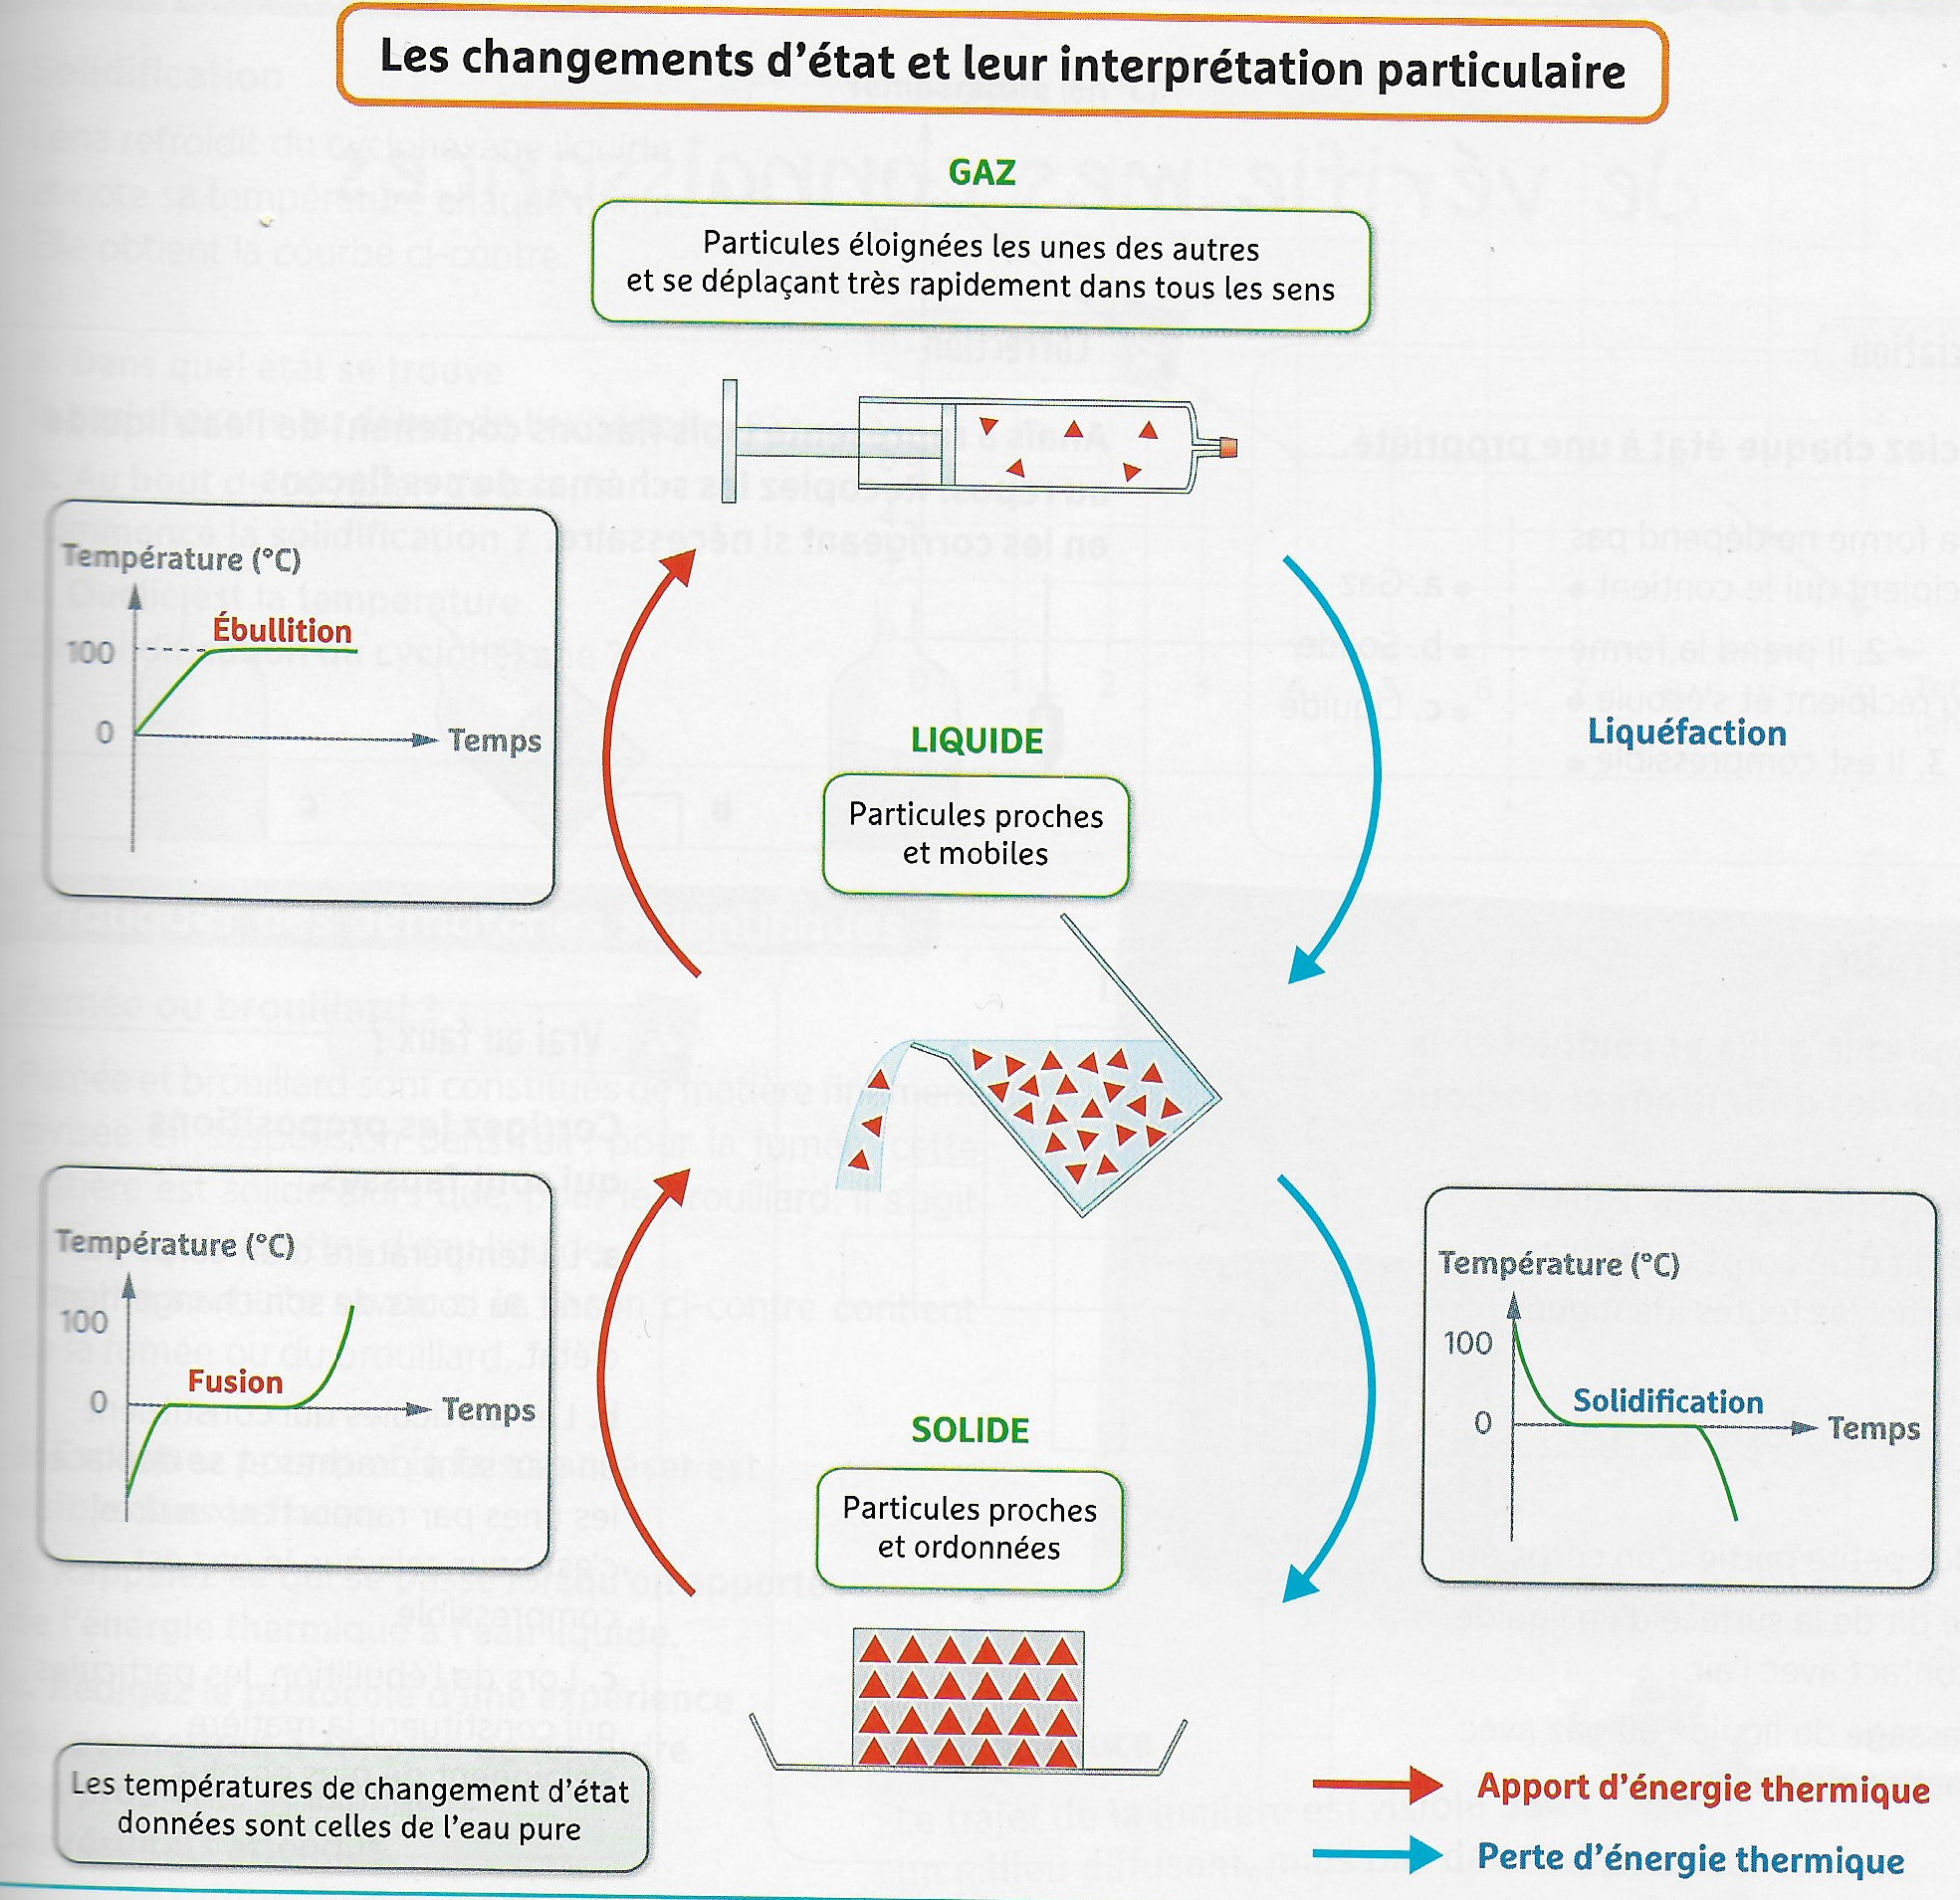
\includegraphics[scale=0.7]{img/chgmt_etats}
	\end{center}
\end{mybilan}